Hopfield-Netze gehen auf den amerikanischen Physiker John Hopfield zurück, der sie zu Beginn der 80er Jahre populär gemacht hat und damit entschieden zur Renaissance Neuronaler Netze Mitte der 80er Jahre beigetragen hat. Es handelt sich dabei um ein weiteres Beispiel für \emph{überwachte} lernende Neuronale Netze.



% ------------------------------------------------------------------------
% ------------------------------------------------------------------------
\section*{Idee}
Die Idee für die Hopfield-Netze ist aus dem Verhalten von Teilchen im Magnetismus entstanden: Jedes Teilchen "`redet"' (durch die magnetischen Kräfte) mit jedem anderen (Vollverknüpfung), wobei es aber jeweils versucht, einen energetisch günstigen Zustand (sozusagen ein \emph{Minimum der Energiefunktion}) zu erreichen. Diesen Eigenzustand kennen wir bei Neuronen als \emph{Aktivierung}.

Nach dieser Idee drehen sich alle Teilchen bzw. Neurone und animieren sich dadurch wieder gegenseitig zur Drehung. Das Neuronales Netz ist also sozusagen eine Wolke von Teilchen.

Ausgehend von der Tatsache, dass die Teilchen die Minima in der Energiefunktion selbsttätig aufspüren, hatte Hopfield nun die Idee, den "`Drehwinkel"' der Teilchen zu nutzen, um Informationsverarbeitung zu betreiben: Warum nicht die Teilchen auf selbstdefinierten Funktionen Minima suchen lassen? Selbst wenn wir nur zwei dieser Drehwinkel (\emph{Spins}) verwenden, also eine binäre Aktivierung, werden wir feststellen, dass das entwickelte Hopfield-Netz erstaunliche Dynamik besitzt.


Abbildung \ref{fig:ch09_hopfield} zeigt ein beispielhaftes Hopfield-Netz. Es besteht aus \emph{einer Schicht Neuronen}, in der jedes Neuron mit allen anderen Neuronen verbunden ist, jedoch \emph{nicht mit sich selbst}.

\begin{figure}[ht!] \centering 
	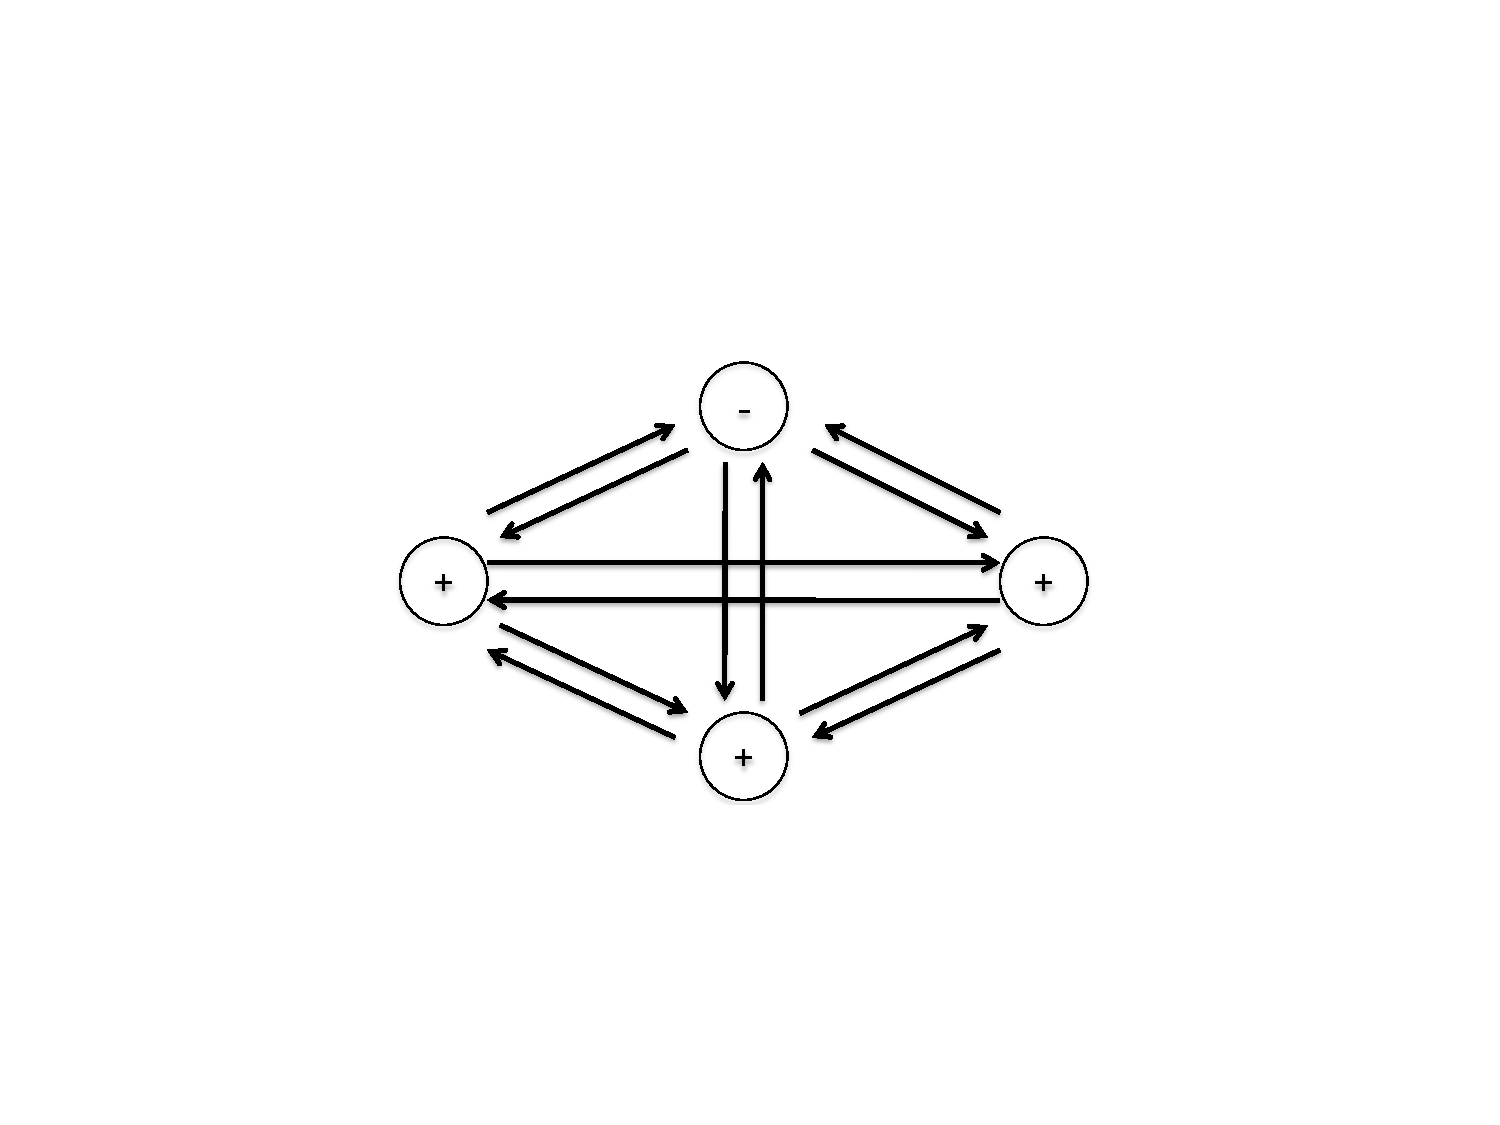
\includegraphics[width=\linewidth]{figures/ch09_hopfield.pdf}
	\caption{Beispielhaftes Hopfield-Netz. Die Markierungen $+$ und $-$ markieren die binären "`Drehwinkel"'. Nummeriert man die Neuronen im Uhrzeigersinn, beginnend beim oberen Neuron, dann ist der Netzzustand $\vec{u} = (-,+,+,+)$.}
	\label{fig:ch09_hopfield}
\end{figure}

Zu sehen sind die \emph{indirekten Rückkopplungen} zwischen je zwei \emph{verschiedenen} Knoten $i$ und $j$, jedoch keine direkten Rückkopplungen zum gleichen Knoten. Ein Hopfield-Netz besteht damit aus einer Menge $K$ von untereinander vollverknüpften Neuronen mit binärer Aktivierung (es werden nur zwei Drehwinkel verwendet), wobei die Gewichte zwischen den einzelnen Neuronen symmetrisch sind ($w_{ij} = w_{ji}$).

Der Zustand von $|K|$ vielen Neuronen mit zwei möglichen Zuständen $\in \{+,-\}$ lässt sich als Zeichenkette $x \in \{+,-\}^|K|$ oder als Vektor $\vec(u) = (u_1, u_2, \ldots, u_{|K|})^T$ beschreiben.


\subsection*{Ein- und Ausgabe}
Die Vollverknüpfung sorgt dafür, dass es weder Eingabe- noch Ausgabeneuronen gibt. Die Eingabe eines Hopfield-Netzes ist ebenso ein Zustand und wird als Zeichenkette $x$ oder Vektor $\vec{u}$ dargestellt.
Das Netz sucht dann zur Eingabe das Minimum auf seiner Energieoberfläche (welches durch Eingabe von Trainingsbeispielen antrainiert wurde).
Das Minimum ist dann erreicht, wenn das Netz \emph{stillsteht}\footnote{Man kann beweisen, dass ein Hopfield-Netz mit symmetrischer Gewichtsmatrix und Nullen in der Diagonale immer konvergiert, es wird also irgendwann still stehen.}.
Die Ausgabe ist dann wieder eine Zeichenkette oder ein Vektor.


\subsection*{Bedeutung der Gewichte}
Neuronen ändern ihre Ausrichtung/Drehung ($+$ oder $-$) ab"-hängig von den aktuellen Zuständen der anderen Neuronen und von den Gewichten zu diesen. Die Gewichte sind damit in der Lage die Gesamtveränderung des Netzes zu steuern.
Dabei gilt:
\begin{itemize}
	\item \emph{positives} Gewicht $w_{ij}$ - Das Gewicht versucht beide Neuronen $i$ und $j$ zur \emph{Gleichheit} zu zwingen. Je größer $w_{ij}$ ist,desto größer der Zwang.
	\item \emph{negatives} Gewicht $w_{ij}$ - Das Gewicht versucht die Neuronen $i$ und $j$ zu \emph{Unterschiedlichkeit} zu zwingen.
	\item \emph{Null-Gewichte} - Sorgen dafür, dass sich die beiden Neuronen nicht beeinflussen.
\end{itemize}

Die Gesamtheit der Gewichte beschreibt den Weg zum nächsten Minimum der Energiefunktion vom aktuellen Netzzustand aus.


\subsection*{Energie}
% Quelle: https://www.youtube.com/watch?v=iQu1ZgmapJQ&list=PLnnr1O8OWc6br8B9iXYFkVJcMc9OnjoZS
Die Gesamtenergie des Netzes ist die Summe des Produktes eines Verbindungsgewichts $w_{ij}$ und den binären Zuständen $s_i$ und $s_j$ zweier Neuronen $i$ und $j$:
\[
	E = - \sum_{i<j} s_i \cdot s_j \cdot w_{ij} - 
		\underbrace{\sum_i s_i \cdot b_i}_{Bias}
\]
Die einfache quadratische Fehlerfunktion ermöglicht es den Einfluss eines einzlenen Neurons auf die Gesamtenergie \emph{lokal} zu berechnen:
\[
	\Delta E_i = E(s_i = 0) - E(s_i = 1) = b_i + \sum_j s_j \cdot w_{ij}
\] 

\subsection*{Zustandsänderungen}
Die Funktionsweise des einmal trainierten und mit einem Anfangszustand initialisierten Netzes liegt darin, die Zustände $x_k$ der einzelnen Neuronen $k$ mit jedem Zeitschritt nach dem folgenden Schema zu ändern.
\[
	x_k(t) = f_{act}\Big( \sum_{j \in K} w_{jk} \cdot x_j(t-1) \Big)
\]
Dabei wird als Aktivierungsfunktion $f_{act}$ in der Regel die Schwellenwert-Funktion mit Schwellenwert $\theta = 0$ verwendet.

Auffallend ist die \emph{asynchrone Aktualisierung}: Es wird jedes mal ein Neuron $k$ zufällig gewählt, welches dann die Aktivierung neu errechnet. Implementiert wird dennoch häufig ein zyklischen Durchlaufen aller Neuronen $K$.




% ------------------------------------------------------------------------
% ------------------------------------------------------------------------
\section*{Training}
Für das Training eines Hopfield-Netzes wird jedes Trainingsmuster $p \in \{1,-1\}^{|K|}$ \emph{genau einmal} angelegt (\emph{Single Shot Learning}).\footnote{Dabei steht die 1 für $+$ und die -1 für $-$.}
Die Gewichte werden dann für alle $p \in P$ wie folgt trainiert:
\[
	w_{ij} = \sum_{p \in P} p_i \cdot p_j
\]
Dabei sind $p_i$ und $p_j$ die Zustände der Neuronen $i$ und $j$ im Beispiel $p$. Daraus ergibt sich die Gewichtsmatrix $W$.

Ein Gewicht $w_{ij}$ berechnet sich als dadurch, in dem für jedes Trainingsmuster $p \in P$ geprüft wird, ob die Neuronen $i$ und $j$ im gleichen Zustand sind. Ist dies der Fall, so wird auf das Gewicht eine $1$ addiert, sind die Zustände verschieden eine $-1$.
Dieser Vorgang wird für alle Gewichte der Gewichtsmatrix $W$ durchgeführt. Anschließend haben diejenigen Gewichte $w_{ij}$ hohe Werte, bei denen $i$ und $j$ bei vielen Trainingsmustern übereingestimmt haben.
Der hohe Wert sagt diesen Neuronen umgangssprachlich: "`Es ist sehr oft energetisch günstig, wenn ihr den gleichen Zustand innehabt."' Entsprechendes gilt für negative Gewichte.

Durch dieses Training kann eine feste Anzahl von Mustern $p$ in der Gewichtsmatrix abgespeichert werden. Das Netz wird dann im trainierten Zustand bei einer Eingabe $x$ zu dem abgespeicherten Muster konvergieren, das der Eingabe $p$ am nächsten liegt.

Leider ist die Zahl der maximal speicherbaren und rekonstruierbaren Muster $p$ auf
\[
	|P|_{MAX} \approx 0.139 \cdot |K|
\]
\noindent
beschränkt.




% ------------------------------------------------------------------------
% ------------------------------------------------------------------------
\section*{Anwendung}
Hopfield-Netze, wie sie hier beschrieben wurden, sind sogenannte \emph{Autoassoziatoren}. Ein Autoassoziator $a$ gibt bei Eingabe eines bekannten Musters $p$ genau dieses bekannte Muster wieder aus, es gilt also:
\[
	a(p) = p
\]
Wobei $a$ die Assoziator-Abbildung ist. Zudem, und darin liegt der Vorteil, funktioniert das auch mit Eingaben die in der Nähe von einem Muster liegen:
\[
	a(p + \epsilon) = p
\]
Nimmt man als Mustermenge $P$ beispielsweise Buchstaben oder sonstige Schriftzeichen in Pixelform, so wird das Netz in der Lage sein, deformierte oder verrauschte Buchstaben mit hoher Wahrscheinlichkeit richtig zu erkennen.

Anwendung von Hopfield-Netzen sind daher prinzipiell \emph{Mustererkennung} und \emph{Mustervervollständigung}, so zum Beispiel Ende der 1980er Jahre die Erkennung von Postleitzahlen auf Briefen. Bald sind die Hopfield-Netze aber in den meisten ihrer Anwendungsgebiete von anderen Systemen überholt worden, weshalb sie heute so gut wie überhaupt nicht mehr verwendet werden.



% ------------------------------------------------------------------------
% ------------------------------------------------------------------------
\section*{Kontinuierliche Hopfield-Netze}
Hopfield beschrieb auch eine Version seiner Netze mit kontinuierlichen Aktivierungen. Hier wird die Aktivierung nicht mehr durch die binäre Schwellenwertfunktion berechnet, sondern durch die Fermifunktion mit Temperaturparameter.

Auch hier ist das Netz für symmetrische Gewichtsmatrizen mit Nullen auf der Diagonalen stabil.

Hopfield selbst nennt als Anwendungsbeispiel für kontinuierliche Hopfield-Netze recht gute Lösungen für das NP-vollständige \emph{Travelling Salesman Problem} zu finden.
Nach einem, im Buch \emph{Simulation Neuronaler Netze} von A. Zell beschriebenen Feldversuch kann dieses Statement aber nicht ohne weiteres aufrecht erhalten werden.
Es gibt heute aber ohnehin schnellere Algorithmen, um gute Lösungen für dieses Problem zu finden, weswegen das Hopfield-Netz auch hier keine Anwendung mehr finden kann.

